\documentclass[11pt, a4paper]{article}

\usepackage{graphicx}
\usepackage[a4paper,top=3cm,bottom=2cm,left=2cm,right=2cm,marginparwidth=1.75cm]{geometry}
\usepackage[english]{babel}
\usepackage[utf8x]{inputenc}
\usepackage{subfig}
\usepackage{float}
\usepackage{amsmath}
\usepackage{amssymb}
\usepackage{mhchem}
\usepackage{hyperref}
\usepackage{tikz}
\usepackage{cancel}

\graphicspath{ {./images} }
\newcommand*{\qed}{\hfill\ensuremath{\quad\square}}%
\newcommand*{\rad}{\ensuremath{\,\text{rad}}}
\newcommand*{\R}{\ensuremath{\mathbb{R}}}
\newcommand*{\C}{\ensuremath{\mathbb{C}}}
\renewcommand*{\Re}{\operatorname{Re}}
\renewcommand*{\Im}{\operatorname{Im}}
\renewcommand*{\epsilon}{\varepsilon}
\renewcommand*{\phi}{\varphi}

\makeatletter
\renewcommand*\env@matrix[1][*\c@MaxMatrixCols c]{%
  \hskip -\arraycolsep
  \let\@ifnextchar\new@ifnextchar
  \array{#1}}
\makeatother

\newtheorem{theorem}{Theorem}

%------------------------------------------------
%Templates for images and figures
% \begin{figure}[h]
%   \centering
%   \subfloat[caption 1]{{
\includegraphics[width=30mm]{images/placeholder.png}}}%
%   \qquad
%   \subfloat[caption 2]{{
\includegraphics[width=30mm]{images/placeholder.png}}}%
%   \caption{Description}
% \end{figure}

% \begin{figure}[h]
%   \centerline{
\includegraphics[width=50mm]{images/placeholder.png}}
%   \caption{Description}
% \end{figure}

%Template for a simple table 
%\begin{table}[h]
%   \caption{Description} %title of the table
%   \centering % centering table
%   \begin{tabular}{l rr} % creating three columns
%     \hline\hline %inserting double-line
%     & & \\ [0.5ex] % Insert half line vertical spacing
%     \hline % inserts single-line
%     & & \\ 
%     & & \\
%     & & \\
%     & & \\
%   \hline % inserts single-line
%   \end{tabular}
%   \label{tab:hresult}
% \end{table}
%-----------------------------------------------

\begin{document}
\setcounter{section}{11}
\setcounter{equation}{0}

\section{Linear Algebra 2 Lecture 12: Singular value decomposition (05/06/2020)}



\subsection{Singular values}
Consider the following matrix transformation $A$ applied to  a unit circle.

\begin{figure}[H]
  \centerline{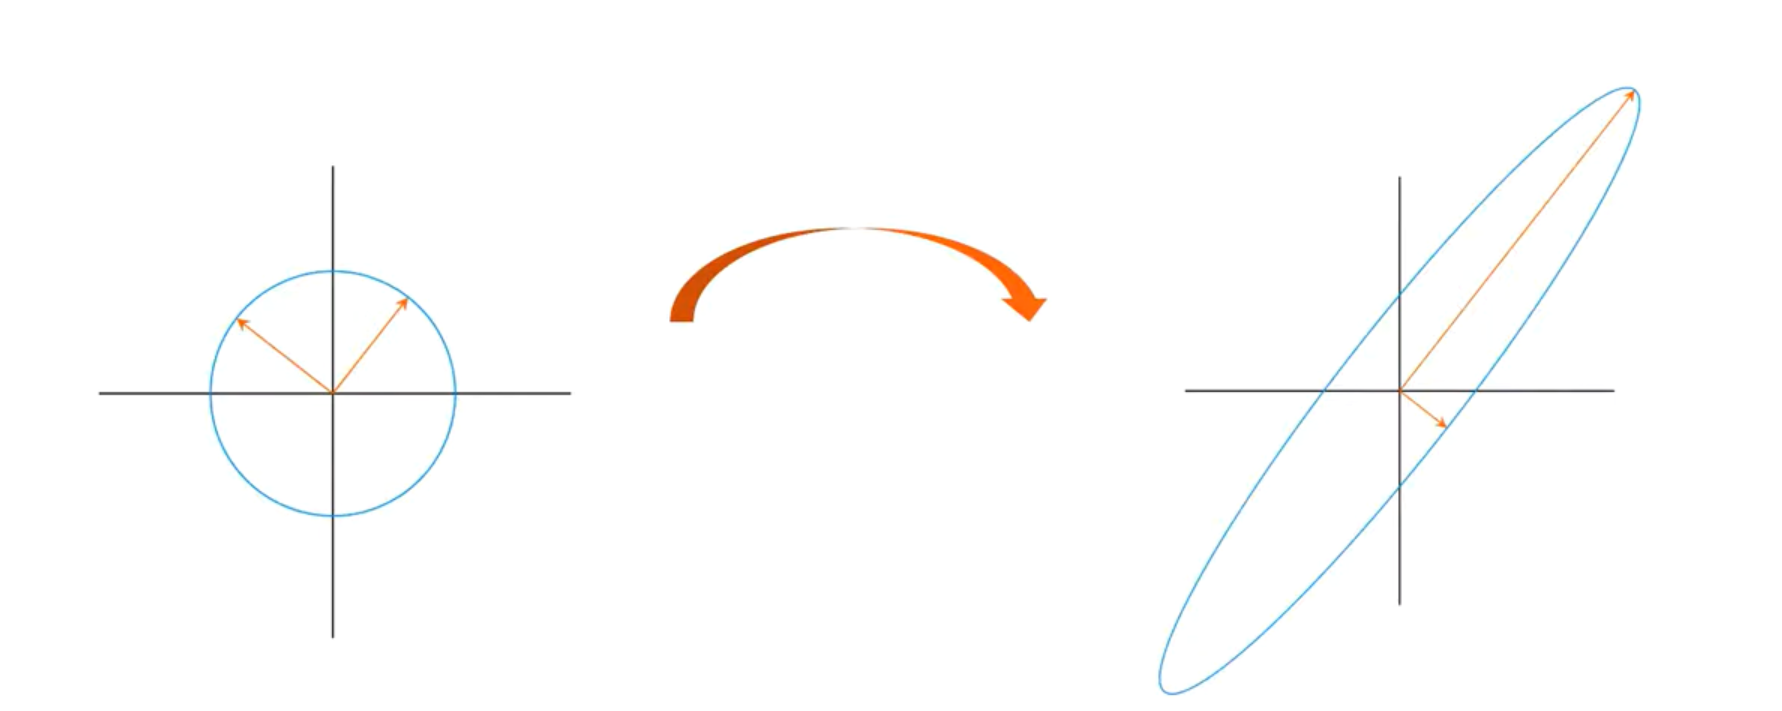
\includegraphics[width=100mm]{images/Transformation.png}}
  \caption{How the unit circle changes to an ellipse under the linear transformation of matrix $A$}
\end{figure}

Where the matrix $A$ is given as:

\begin{equation}
	A = 
	\begin{bmatrix}
		1 & 2\\
		2 & 2\\
	\end{bmatrix}
\end{equation}

The semi-major axis for the created ellipse will be $|\lambda_{max}| = \frac{1}{2}(3 + \sqrt{17})$. The semi-minor axis will then be given as: $|\lambda_{min}| = \frac{1}{2}(\sqrt{17} - 3)$. Let's now consider a more tricky situation. We start with a unit sphere in $\R^3$. We then map this sphere to an ellipse on a 2 diminsional plane. The matrix $A$ for this transformation will be:

\begin{equation}
	A =
	\begin{bmatrix}
		4 & 11 & 14\\
		8 & 7 & -2\\
	\end{bmatrix}
\end{equation}

\begin{figure}[H]
  \centerline{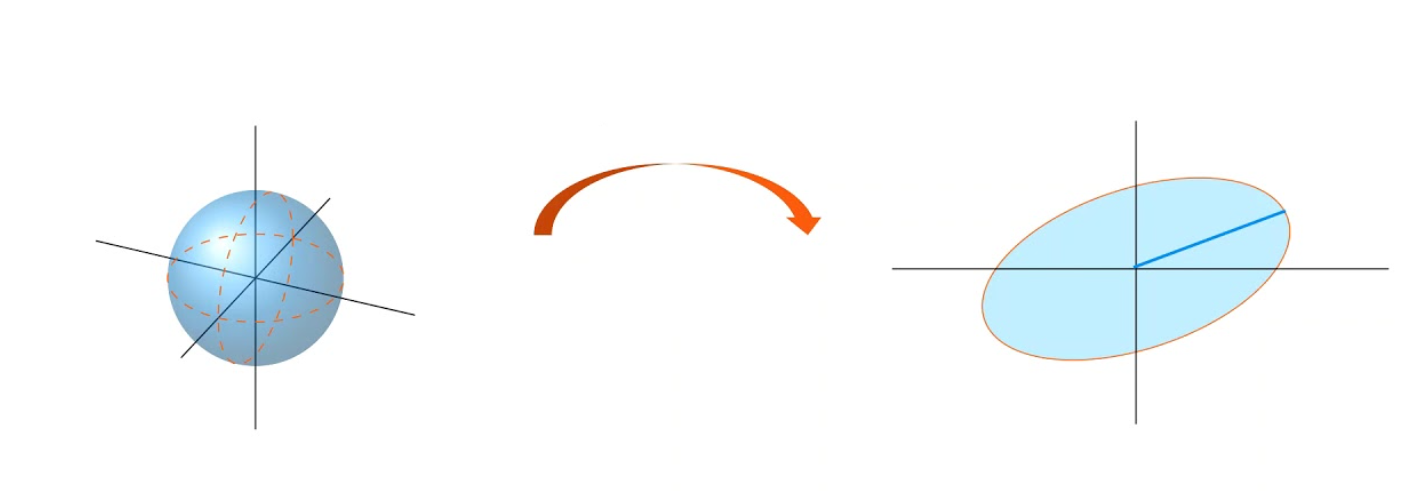
\includegraphics[width=100mm]{images/Transformation_2.png}}
  \caption{How the unit sphere changes to an ellipse on a 2D plane under the linear transformation of matrix $A$}
\end{figure}

Simply finding the eigenvalues of the matrix $A$ is not going to work, as non-square matrices do not have eigenvalues. We can instead turn this problem into a constraint optimization problem. We consider the unit sphere a constraint $||\vec{x}|| = 1$. We then look for the minimum and maximum values a given vector gets after applying the linear transformation $A$. In other words we want to maximize $||A\vec{x}||$. This is the same as maximizing $||A\vec{x}||^2$. Hence the problem becomes:\\
\\
\centerline{Maximize $||A\vec{x}||^2$ under the constraint $\vec{x}=1$.}\\
\\
This is just a quadratic form which we know how to solve. The maximum occurs at the maximum value of the eigenvalue of the matrix $A^TA$, which is square by definition of the matrix product and thus has eigenvalues. Somce we spolved for $||A\vec{x}||^2$ rather then for $||A\vec{x}||$ the semi-major and semi-minor axis become:

\begin{gather}
	\sqrt{\lambda_{max}} = 6\sqrt{10}\\
	\sqrt{\lambda_{min}} = 3\sqrt{10}
\end{gather}

For every $m \times n$ matrix $A$ all eigenvalues of the symmetric $A^TA$ are non-negative. To prove thsi consider the following: $\lambda$ is an eigenvalue of $A^TA$ corresponding to $\vec{v}$ with the cosntraint that $||\vec{v}|| = 1$. Then:

\begin{equation}
	\lambda = \vec{v}^T\lambda \vec{v} = \vec{v}^T A^T A \vec{v} = A\vec{v} \cdot A \vec{v} = ||A\vec{v}||^2 \geq 0
\end{equation}

These square roots of the eigenvalues of $A^TA$ are called the singular values of $A$. They are defiend as follows: The singular values of an $m \times n$ matrix $A$ are the square roots of the eigenvalues of $A^TA$, usually denoted as $\sigma_1, \sigma_2, \cdots, \sigma_n$ and arranged in decreasing order.



\subsection{Orthogonal basis of Col($A$)}
Suppose that $\lambda_1 \geq \cdots \geq \lambda_r > 0$ and that $\lambda_{r+1} = \cdots = \lambda_n = 0$ are the eigenvalues of$A^TA$. Let $\{\vec{v}_1, \cdots, \vec{v}_n \}$ be an orthonormal set corresponding to the eigenvalues. Then $\{A\vec{v}_1, \cdots, A\vec{v}_n \}$ is an orthogonal basis for the basis of Col($A$). Hence $r$, the number of non-zero singular values of $A$, is equal to the rank($A$) = dim(Col($A$)).



\subsection{The singular value decomposition}
Let $A$ be an $m \times n$ matrix of rank $r$. Then $A = U\Sigma V^T$, where:

\begin{itemize}
	\item $U$ is an orthogonal $m \times m$ matrix
	\item $V$ is an orthogonal $n \times n$ matrix
	\item $\Sigma$ is an $m \times n$ matrix consisting of the non-zero singular values of $A$ and $0$ entries.
\end{itemize}

\begin{equation}
	\Sigma = 
	\begin{bmatrix}[ccc|c]
		\sigma_1 & \cdots & 0 & \\
		\vdots & \ddots & \vdots & O\\
		0 & \cdots & \sigma_r & \\
		\hline
		& O & & O
	\end{bmatrix}
\end{equation}

To find $V$ we find an orthogonal diagonalization of $A^TA$, arranging its eigenvalues in decreasing order. If $A^TA = PDP^T$ we define $P=V$. For the matrix $U$:
\begin{equation}
	\vec{u}_i = \frac{1}{\sigma_i} A \vec{v}_i, \quad \text{for}\; i=1,\cdots, r
\end{equation}
$\vec{v}_i$ refers to the $i$-th column of $V$. We extend $\{\vec{u}_1 \cdots \ vec{u}_r \}$ to be an orthonormal basis $\{\vec{u}_1 \cdots \ vec{u}_m \}$ for $\R^m$ and define the columns of $U$ as:
\begin{equation}
	U = 
	\begin{bmatrix}
		\vec{u}_1 & \cdots & \vec{u}_m
	\end{bmatrix}
\end{equation}
if $A=U\Sigma V^T$ is a singular value decomposition of $A$, then $A^T = V\Sigma U^T$ is a singular value decomposition of $A^T$. Since $A$ and $A^T$ share the same characteristic polynomial they also share the same eigenvalues and by extension the same singular values. The columns of $V$ form an orthonormal set of eigenvectors of $A^T A$ and the columns of $U$ for an orthonormal set of eigenvectors of $AA^T$.



\subsection{The four fundamental subspaces}
if $A=U\Sigma V^T$ is a singular value decomposition of $A$, then:
\begin{itemize}
	\item $\{ \vec{u}_1, \cdots, \vec{u}_r \}$ is an orthonormal basis for Col($A$)
	\item $\{ \vec{u}_{r+1}, \cdots, \vec{u}_m \}$ is an orthonormal basis for Nul($A^T$)=$(\text{Col}(A))^\perp$
	\item $\{ \vec{v}_1, \cdots, \vec{v}_r \}$ is an orthonormal basis for Col($A^T$)
	\item $\{ \vec{u}_{r+1}, \cdots, \vec{v}_n \}$ is an orthonormal basis for Nul($A$)
\end{itemize}


\end{document}